\section{Data Analysis - In Depth}

\subsection{Data Analysis}\label{ftml-jrnl:sec:dataanalysis}

%	\begin{figure}[tbp]
%	    \centering
%	    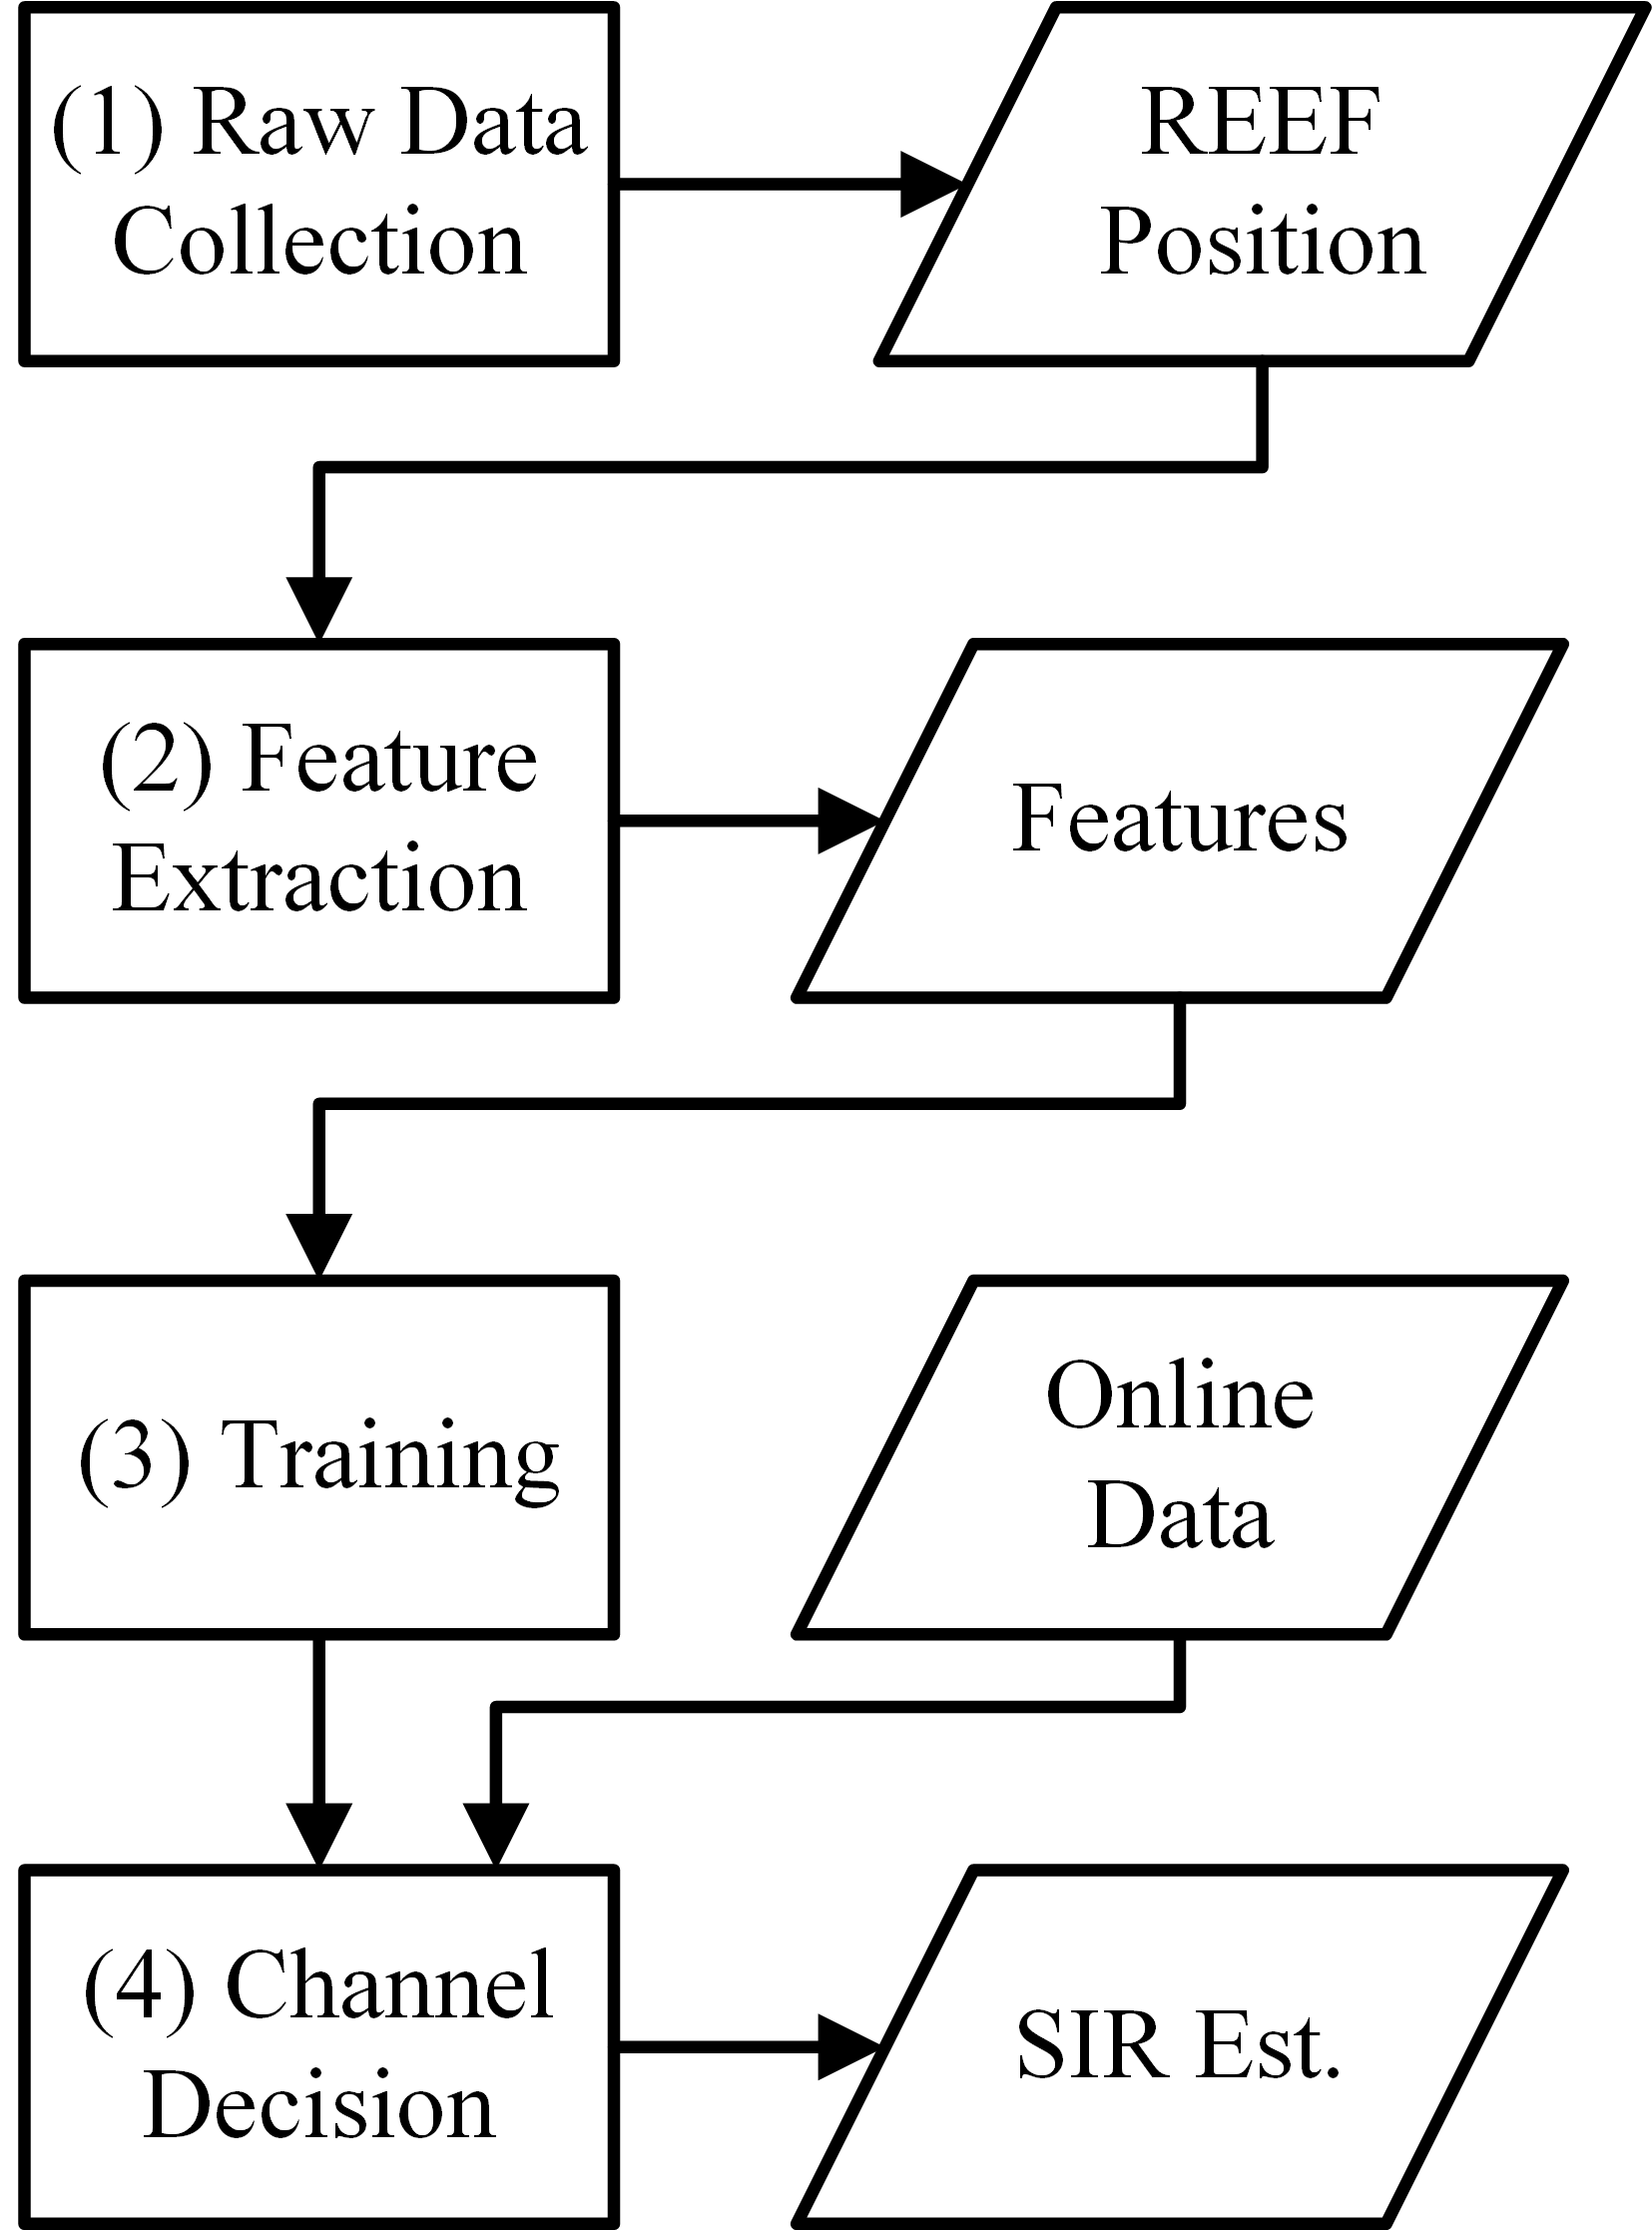
\includegraphics[width=0.65\columnwidth]{diagrams/DataFlow-verticle}
%	    \caption{Data analytics includes raw data capture from a vision system, feature extraction, training, and  operation.}
%	    \label{ftml-jrnl:fig:dataflow}
%	\end{figure}

The data analysis process for the experiment
%was conducted according to the diagram in Fig.~\ref{ftml-jrnl:fig:dataflow} and 
is divided into four parts: raw data collection, data cleaning and feature extraction, training, and the operation of the SIR estimation. The raw data was produced as an output of the VTS as a time series of z-axis position. Feature extraction was conducted in MATLAB by following the time series and extracting or calculating features for each iteration.  Once features were extracted, a statistical analysis of the features was conducted to determine the variability of the features as a function of SIR \cite{Candell_ISIT_2019}. Training of a machine learning algorithm followed. The machine learning algorithm was programmed in Python using the Sci-kit Learn library~\cite{SCIKITLEARN}.

\subsubsection{Feature Extraction}\label{ftml-jrnl:sec:data:feats}

%\begin{figure}[tbp]
%	\centering
%	\subfloat[sample time series of probe position in mm\label{ftml-jrnl:fig:timeseries-zplot}]{%
%		\includegraphics[width=0.75\columnwidth]{plots/timeseries-zplot}}
%	\hfill
%	\subfloat[feature extraction model\label{ftml-jrnl:fig:timeseriesfeatures}]{%
%		\includegraphics[width=0.8\columnwidth]{diagrams/timeseries.png}}
%	\caption{A time-series sample~\subref{ftml-jrnl:fig:timeseries-zplot} of a single iteration of the measured z-axis probe position and~\subref{ftml-jrnl:fig:timeseriesfeatures} the corresponding model for feature extraction.}
%	\label{ftml-jrnl:fig:timeseries-and-model}      
%\end{figure}

\begin{figure}[!ht]
	\centering
	
	\begin{subfigure}{.75\textwidth}
		\centering
		% include first image
		\includegraphics[width=.8\linewidth]{./chapter-ftml/plots/timeseries-zplot}  
		\caption{sample time series of probe position in mm}
		\label{ftml-jrnl:fig:timeseries-zplot}
	\end{subfigure}

	\begin{subfigure}{.75\textwidth}
		\centering
		% include second image
		\includegraphics[width=.8\linewidth]{./chapter-ftml/diagrams/timeseries.png}  
		\caption{feature extraction model}
		\label{ftml-jrnl:fig:timeseriesfeatures}
	\end{subfigure}

	\caption{A time-series sample~\protect\subref{ftml-jrnl:fig:timeseries-zplot} of a single iteration of the measured z-axis probe position and~\protect\subref{ftml-jrnl:fig:timeseriesfeatures} the corresponding model for feature extraction.}
	\label{ftml-jrnl:fig:timeseries-and-model}
	
\end{figure}	

A sample time series of the z-axis position of the probe is as shown in~Fig.~\ref{ftml-jrnl:fig:timeseries-zplot}.  Rather than using the time series directly, a more convenient and practical solution is to extract features that represent aspects that may be useful for analysis and machine learning algorithms. The selected features are illustrated in~Fig.~\ref{ftml-jrnl:fig:timeseriesfeatures}. Shown in the model, the probe begins at its home position, \textbf{a}.  It will not begin its downward motion until it receives sufficient FTS readings.  Marker \textbf{b} indicates the beginning of the probes descent.  Marker \textbf{c} represents that point in which the probe descends below a predetermined threshold, and marker \textbf{d} represents the position in which the probe begins its return ascent to the home position.  Finally the probe returns to the home position as indicated by marker \textbf{e}.  Therefore, the extracted features of each successive iteration is defined as follows:

\begin{description}
	\item[Feature $Z_d$] The length of the probe's descent measured in millimeters,
	\item[Feature $\Delta{t}_{ab}$] The duration in seconds the the robot waits before moving the probe along its descent,
	\item[Feature $\Delta{t}_{bc}$] The duration in seconds of the time that the robot takes to move the probe beyond the threshold, $Z_{th}$, of -77 mm,
	\item[Feature $\Delta{t}_{cd}$] The duration in which the probe dwells below $Z_{th}$ and the speed of the probe remains under 0.15 mm/sec,
	\item[Feature $\Delta{t}_{ae}$] The duration of the full iteration as measured from the home position, \textbf{a}, to the next home position, \textbf{e}.
\end{description}

\subsubsection{ML-based SIR Estimation}\label{ftml-jrnl:sec:data:ML}
In order to learn the SIR level from observing the various features, we can leverage supervised machine learning regression schemes. 
%the random forest model \cite{RF}. Random forest is an ensemble of decision trees with random feature selection which can be used for classification or regression based on the predicted output space. Deploying random forest in machine learning has been successful in various applications such as \cite{RF_1,RF_2,RF_3}. Its main advantages are that it is stable, fast to compute, and insusceptible to over-fitting.
In this work, we compare the deployment of various machine learning algorithms for SIR regression using the five features defined in \ref{ftml-jrnl:sec:data:feats}. These features are evaluated for each iteration of the probe movement. We define a data segment which is composed of a number of successive iterations and we denote the segment size by $M$. As a result, we use each regression model to get an input vector of size $5M$ and the regression output of the corresponding SIR value. 
%The random forest is selected because it is computationally efficient with high-dimensional data and it is robust for outliers and data non-linearity. 

We start by training each regression model by taking a fixed number of segments for each SIR labelled data. We denote the size of the training set for each SIR level by $T$. The rest of the measurements are used for testing. In general, the proposed machine learning approach will deploy a sliding window approach of size $M$ to collect the features of the force-seeking use case to estimate the current level of SIR at various nodes of the wireless network. 

\subsection{Results} \label{ftml-jrnl:sec:results}  
In this section, we consider the experimental results for 4 different settings. The dataset of all the collected data is available online~\cite{https://doi.org/10.18434/m32077}. The four settings are defined as follows: i) setting b/g-Router: the jamming signal impacts the router and IEEE 802.11 b/g is deployed ~\cite{IEEE802.11ac}, ii) setting b/g-Station: the jamming signal impacts the station and IEEE 802.11 b/g is deployed, iii) setting b/g/n-Router: the jamming signal impacts the router and IEEE 802.11 b/g/n is deployed, and iv) setting b/g/n-Station: the jamming signal impacts the station and IEEE 802.11 b/g/n is deployed.  

When the jamming signal has an impact on the router, we consider 3 values of the SIR which are -9, -8, -7 dB while having 1, 2, 3 dB for the settings in which jamming has an impact on the station. Except otherwise mentioned, we set$M = 50$ and $T = 200$. 

\subsubsection{Machine Learning Algorithm Comparison}
In this subsection, we compare various regression approaches using two performance criteria, namely, the mean squared error (MSE) and the R-squared variance score \cite{r-squared}. R-squared variance score indicates the percentage of the variance in the dependent variable that the independent variables explain collectively. The used version of R-squared in the Sci-kit Learn library measures the strength of the relationship between your model and the dependent variable on a convenient -1 to 1 scale. The best possible outcome is 1 when predicted values capture the variance of the independent variable. It takes a value of 0 when the predicted value is constant and negative values when the regression model cannot follow the trend of the data. We present the performance for different values of $M$. The compared algorithms are the random forest, gradient boosting, extreme gradient boosting (XGBM), decision tree, support vector machine (SVM), k-nearest neighbor, kernel ridge, and linear ridge \cite{SCIKITLEARN,Chen:2016:XST:2939672.2939785}. %xxxx references needed

% Table generated by Excel2LaTeX from sheet 'ML_Regression_MSE'
\begin{table}[!ht]
	\centering
	\caption{MSE values of various ML algorithms for jamming setting b/g-Router}
	\begin{tabular}{|p{5.3em}|c|c|c|c|c|}
		\toprule
		& \multicolumn{1}{p{2.4em}|}{M = 1} & \multicolumn{1}{p{2.9em}|}{M = 10} & \multicolumn{1}{p{2.9em}|}{M = 30} & \multicolumn{1}{p{2.9em}|}{M = 50} & \multicolumn{1}{p{3.4em}|}{M = 100} \\
		\midrule
		Random Forest	 & 0.61  & 0.54  & 0.49  & 0.48  & 0.46 \\
		\midrule
		Gradient Boosting  & 0.56  & 0.55  & 0.47  & 0.45  & 0.44 \\
		\midrule
		XGBM  & 0.62  & 0.53  & 0.45  & 0.43  & 0.41 \\
		\midrule
		Decission Tree & 1.07  & 0.99  & 0.87  & 0.91  & 0.97 \\
		\midrule
		SVM   & 0.92  & 0.99  & 0.98  & 0.97  & 0.96 \\
		\midrule
		KNN   & 0.73  & 0.74  & 0.73  & 0.74  & 0.77 \\
		\midrule
		Kernal Ridge & 0.97  & 0.73  & 0.71  & 0.71  & 0.71 \\
		\midrule
		Linear Ridge & 0.7   & 0.7   & 0.7   & 0.71  & 0.71 \\
		\bottomrule
	\end{tabular}%
	\label{ftml-jrnl:tab:T1}%
\end{table}%

In Table~\ref{ftml-jrnl:tab:T1}, we present the MSE performance of various algorithms at setting b/g-Router. The ensemble-based algorithms, which are the random forest, gradient boosting, and XGBM, perform better than non-ensemble algorithms. This happens because the ensemble-based algorithms learn from the training data without having an initial model to fit thus allowing for capturing the randomness impacts on the collected data. Moreover, the XGBM gives slightly better performance than the random forest and gradient boosting algorithms except at $M=1$. The XGBM performs gradient boosting over random set of trees and hence the superior performance. We also find it has superior variance score as well in Table~\ref{ftml-jrnl:tab:T2}. Generally, in Table~\ref{ftml-jrnl:tab:T2}, similar trends as Table~\ref{ftml-jrnl:tab:T1} can be found for various machine learning algorithms where ensemble-based algorithms have the best performance among others and their performance is enhanced by increasing the segment size $M$ of the measured data.

% Table generated by Excel2LaTeX from sheet 'ML_Regression_R2'
\begin{table}[!ht]
	\centering
	\caption{Variance score values of various ML algorithms for jamming setting b/g-Router}
	\begin{tabular}{|p{5.3em}|c|c|c|c|c|}
		\toprule
		& \multicolumn{1}{p{2.4em}|}{M = 1} & \multicolumn{1}{p{2.9em}|}{M = 10} & \multicolumn{1}{p{2.9em}|}{M = 30} & \multicolumn{1}{p{2.9em}|}{M = 50} & \multicolumn{1}{p{3.4em}|}{M = 100} \\
		\midrule
		Random Forest	 & 0.15  & 0.2   & 0.3   & 0.35  & 0.35 \\
		\midrule
		Gradient Boosting  & 0.02  & 0.2   & 0.34  & 0.37  & 0.42 \\
		\midrule
		XGBM  & 0.12  & 0.25  & 0.36  & 0.4   & 0.43 \\
		\midrule
		Decission Tree & -0.57 & -0.44 & -0.36 & -0.3  & -0.22 \\
		\midrule
		SVM   & -0.34 & -0.38 & -0.37 & -0.37 & -0.32 \\
		\midrule
		KNN   & -0.05 & -0.02 & -0.02 & -0.08 & -0.04 \\
		\midrule
		Kernal Ridge & -0.48 & -0.05 & 0     & 0     & 0 \\
		\midrule
		Linear Ridge & 0.01  & 0.01  & 0     & -0.01 & 0 \\
		\bottomrule
	\end{tabular}%
	\label{ftml-jrnl:tab:T2}%
\end{table}%


% Table generated by Excel2LaTeX from sheet 'ML_Regression_MSE'
% \begin{table}[htbp]
%   \centering
%   \caption{MSE Values of various ML algorithms for setting 2}
%     \begin{tabular}{|p{6.7em}|c|c|c|c|c|}
%     \toprule
%           & \multicolumn{1}{p{3em}|}{M = 1} & \multicolumn{1}{p{3em}|}{M = 10} & \multicolumn{1}{p{3em}|}{M = 30} & \multicolumn{1}{p{3em}|}{M = 50} & \multicolumn{1}{p{3.5em}|}{M = 100} \\
%     \midrule
%     Random Forest	 & 0.31  & 0.23  & 0.2   & 0.18  & 0.17 \\
%     \midrule
%     Gradient Boosting  & 0.32  & 0.16  & 0.14  & 0.14  & 0.14 \\
%     \midrule
%     XGBM  & 0.3   & 0.17  & 0.12  & 0.1   & 0.1 \\
%     \midrule
%     Decission Tree & 0.6   & 0.48  & 0.46  & 0.44  & 0.39 \\
%     \midrule
%     SVM   & 0.96  & 0.96  & 0.94  & 0.95  & 0.88 \\
%     \midrule
%     KNN   & 0.76  & 0.73  & 0.7   & 0.71  & 0.73 \\
%     \midrule
%     Kernal Ridge & 4.9   & 1.08  & 0.69  & 0.44  & 0.39 \\
%     \midrule
%     Linear Ridge & 0.67  & 0.67  & 0.67  & 0.67  & 0.66 \\
%     \bottomrule
%     \end{tabular}%
%   \label{ftml-jrnl:tab:addlabel}%
% \end{table}%

% % Table generated by Excel2LaTeX from sheet 'ML_Regression_R2'
% \begin{table}[htbp]
%   \centering
%   \caption{variance Score Values of various ML algorithms for setting 2}
%     \begin{tabular}{|p{6.7em}|c|c|c|c|c|}
%     \toprule
%           & \multicolumn{1}{p{3em}|}{M = 1} & \multicolumn{1}{p{3em}|}{M = 10} & \multicolumn{1}{p{3em}|}{M = 30} & \multicolumn{1}{p{3em}|}{M = 50} & \multicolumn{1}{p{3.5em}|}{M = 100} \\
%     \midrule
%     Random Forest	 & 0.54  & 0.69  & 0.74  & 0.74  & 0.76 \\
%     \midrule
%     Gradient Boosting  & 0.49  & 0.71  & 0.8   & 0.79  & 0.81 \\
%     \midrule
%     XGBM  & 0.56  & 0.77  & 0.83  & 0.85  & 0.85 \\
%     \midrule
%     Decission Tree & 0.14  & 0.31  & 0.34  & 0.36  & 0.35 \\
%     \midrule
%     SVM   & -0.45 & -0.39 & -0.46 & -0.43 & -0.36 \\
%     \midrule
%     KNN   & -0.08 & -0.06 & -0.07 & -0.11 & -0.09 \\
%     \midrule
%     Kernal Ridge & -5.98 & -0.62 & -0.07 & -0.04 & 0.02 \\
%     \midrule
%     Linear Ridge & 0     & 0     & 0     & 0     & -0.01 \\
%     \bottomrule
%     \end{tabular}%
%   \label{ftml-jrnl:tab:addlabel}%
% \end{table}%

% 	% Table generated by Excel2LaTeX from sheet 'ML_Regression_MSE'
% \begin{table}[htbp]
%   \centering
%   \caption{MSE Values of various ML algorithms for setting 3}
%     \begin{tabular}{|p{6.7em}|c|c|c|c|c|}
%     \toprule
%           & \multicolumn{1}{p{3em}|}{M = 1} & \multicolumn{1}{p{3em}|}{M = 10} & \multicolumn{1}{p{3em}|}{M = 30} & \multicolumn{1}{p{3em}|}{M = 50} & \multicolumn{1}{p{3.5em}|}{M = 100} \\
%     \midrule
%     Random Forest	 & 0.49  & 0.37  & 0.31  & 0.29  & 0.27 \\
%     \midrule
%     Gradient Boosting  & 0.58  & 0.36  & 0.25  & 0.24  & 0.18 \\
%     \midrule
%     XGBM  & 0.53  & 0.35  & 0.25  & 0.2   & 0.15 \\
%     \midrule
%     Decission Tree & 1.03  & 0.84  & 0.82  & 0.69  & 0.73 \\
%     \midrule
%     SVM   & 0.94  & 0.95  & 0.86  & 0.89  & 0.83 \\
%     \midrule
%     KNN   & 0.67  & 0.67  & 0.67  & 0.67  & 0.73 \\
%     \midrule
%     Kernal Ridge & 0.62  & 0.63  & 0.6   & 0.6   & 0.61 \\
%     \midrule
%     Linear Ridge & 0.6   & 0.6   & 0.61  & 0.61  & 0.63 \\
%     \bottomrule
%     \end{tabular}%
%   \label{ftml-jrnl:tab:addlabel}%
% \end{table}%

% 	% Table generated by Excel2LaTeX from sheet 'ML_Regression_R2'
% \begin{table}[htbp]
%   \centering
%   \caption{variance Score Values of various ML algorithms for setting 3}
%     \begin{tabular}{|p{6.7em}|c|c|c|c|c|}
%     \toprule
%           & \multicolumn{1}{p{3em}|}{M = 1} & \multicolumn{1}{p{3em}|}{M = 10} & \multicolumn{1}{p{3em}|}{M = 30} & \multicolumn{1}{p{3em}|}{M = 50} & \multicolumn{1}{p{3.5em}|}{M = 100} \\
%     \midrule
%     Random Forest	 & 0.12  & 0.35  & 5     & 0.5   & 0.56 \\
%     \midrule
%     Gradient Boosting  & 0.02  & 0.39  & 0.53  & 0.6   & 0.67 \\
%     \midrule
%     XGBM  & 0.16  & 0.45  & 0.6   & 0.66  & 0.73 \\
%     \midrule
%     Decission Tree & -0.79 & -0.38 & -0.33 & -0.26 & -0.16 \\
%     \midrule
%     SVM   & -0.56 & -0.6  & -0.55 & -0.52 & -0.41 \\
%     \midrule
%     KNN   & -0.15 & -0.13 & -0.14 & -0.1  & -0.24 \\
%     \midrule
%     Kernal Ridge & -0.41 & -0.04 & -0.01 & -0.02 & -0.03 \\
%     \midrule
%     Linear Ridge & 0     & -0.01 & -0.03 & -0.05 & -0.09 \\
%     \bottomrule
%     \end{tabular}%
%   \label{ftml-jrnl:tab:addlabel}%
% \end{table}%

Similarly, in Table~\ref{ftml-jrnl:tab:T3}, the ensemble-based algorithms perform better than other algorithms and the XGBM is the best among them. In this setting b/g/n-Station, the interference impacts the router and hence the MSE values generally higher than the corresponding cases in setting b/g-Router. In this case, the interference has a larger impact and hence larger MSE. That leads to larger distinction between the performance of the machine learning algorithms. 
% Table generated by Excel2LaTeX from sheet 'ML_Regression_MSE'
\begin{table}[!ht]
	\centering
	\caption{MSE values of various ML algorithms for jamming setting b/g-Station}
	\begin{tabular}{|p{5.3em}|c|c|c|c|c|}
		\toprule
		& \multicolumn{1}{p{2.4em}|}{M = 1} & \multicolumn{1}{p{2.9em}|}{M = 10} & \multicolumn{1}{p{2.9em}|}{M = 30} & \multicolumn{1}{p{2.9em}|}{M = 50} & \multicolumn{1}{p{3.4em}|}{M = 100} \\
		\midrule
		Random Forest	 & 0.88  & 0.79  & 0.76  & 0.69  & 0.7 \\
		\midrule
		Gradient Boosting  & 0.95  & 0.71  & 0.61  & 0.56  & 0.56 \\
		\midrule
		XGBM  & 0.85  & 0.73  & 0.59  & 0.52  & 0.48 \\
		\midrule
		Decission Tree & 1.48  & 1.46  & 1.33  & 1.33  & 1.32 \\
		\midrule
		SVM   & 1.34  & 1.36  & 1.36  & 1.39  & 1.49 \\
		\midrule
		KNN   & 1.01  & 1.04  & 1.03  & 1.05  & 1.13 \\
		\midrule
		Kernal Ridge & 4.42  & 1.25  & 0.98  & 0.97  & 0.99 \\
		\midrule
		Linear Ridge & 0.93  & 0.94  & 0.94  & 0.95  & 0.99 \\
		\bottomrule
	\end{tabular}%
	\label{ftml-jrnl:tab:T3}%
\end{table}%

% 	% Table generated by Excel2LaTeX from sheet 'ML_Regression_R2'
% \begin{table}[htbp]
%   \centering
%   \caption{variance Score Values of various ML algorithms for setting 4}
%     \begin{tabular}{|p{6.7em}|c|c|c|c|c|}
%     \toprule
%           & \multicolumn{1}{p{3em}|}{M = 1} & \multicolumn{1}{p{3em}|}{M = 10} & \multicolumn{1}{p{3em}|}{M = 30} & \multicolumn{1}{p{3em}|}{M = 50} & \multicolumn{1}{p{3.5em}|}{M = 100} \\
%     \midrule
%     Random Forest	 & 0.08  & 0.15  & 0.22  & 0.27  & 0.3 \\
%     \midrule
%     Gradient Boosting  & -0.04 & 0.23  & 0.39  & 0.43  & 0.44 \\
%     \midrule 
%     XGBM  & 0.07  & 0.21  & 0.37  & 0.46  & 0.53 \\
%     \midrule
%     Decission Tree & -0.51 & -0.49 & -0.42 & -0.39 & -0.48 \\
%     \midrule
%     SVM   & -0.44 & -0.51 & -0.44 & -0.46 & -0.52 \\
%     \midrule
%     KNN   & -0.12 & -0.13 & -0.1  & -0.09 & -0.12 \\
%     \midrule
%     Kernal Ridge & -3.61 & -0.26 & -0.05 & 0     & 0 \\
%     \midrule
%     Linear Ridge & 0     & -0.01 & 0     & 0     & 0 \\
%     \bottomrule
%     \end{tabular}%
%   \label{ftml-jrnl:tab:addlabel}%
% \end{table}%

\subsubsection{Tuning the Random Forest and Gradient Boosting Regressors}

In this subsection, we study the impacts of the number of estimators and the depth for gradient boosting and random forest algorithms. The XGBM parameters are optimized automatically when the function is called to be executed. We show the MSE performance results for setting b/g-Router while same trend holds for other system settings as well. 

For random forest algorithm, we show in Table~\ref{ftml-jrnl:tab:T4} that the tree depth has more impact on the performance than the number of the estimators (\# est.). However, increasing the depth improves the performance till the value of 5 where increasing the depth cause slight improvements.   
% Table generated by Excel2LaTeX from sheet 'ML_Random_Forest_MSE_Matrix'
\begin{table}[!ht]
	\centering
	\caption{MSE of Random Forrest regression parameters for jamming setting b/g-Router}
	\begin{tabular}{|c|c|c|c|c|c|c|}
		\toprule
		\backslashbox{Depth}{\# est.}
		
		& 100   & 200   & 300   & 400   & 500   & 600 \\
		\midrule
		1     & 0.64  & 0.64  & 0.64  & 0.63  & 0.63  & 0.63 \\
		\midrule
		3     & 0.53  & 0.53  & 0.53  & 0.53  & 0.53  & 0.52 \\
		\midrule
		5     & 0.5   & 0.5   & 0.5   & 0.48  & 0.48  & 0.48 \\
		\midrule
		7     & 0.49  & 0.49  & 0.48  & 0.48  & 0.48  & 0.48 \\
		\midrule
		9     & 0.48  & 0.48  & 0.47  & 0.47  & 0.47  & 0.47 \\
		\bottomrule
	\end{tabular}%
	\label{ftml-jrnl:tab:T4}%
\end{table}%

For gradient boosting, we show in Table~\ref{ftml-jrnl:tab:T5} that a similar trend as a random forest exists where depth has a larger impact on the performance. However, increasing the depth more than 7 causes the MSE performance to degrade significantly. 

% Table generated by Excel2LaTeX from sheet 'ML_Gradient_Boosting__MSE_Matri'
\begin{table}[!ht]
	\centering
	\caption{MSE of Gradient Boosting regression parameters for jamming setting b/g-Router}
	\begin{tabular}{|c|c|c|c|c|c|c|}
		\toprule
		\backslashbox{Depth}{\# est.}
		& 100   & 200   & 300   & 400   & 500   & 600 \\
		\midrule
		1     & 0.48  & 0.47  & 0.46  & 0.46  & 0.45  & 0.46 \\
		\midrule
		3     & 0.47  & 0.47  & 0.47  & 0.47  & 0.46  & 0.47 \\
		\midrule
		5     & 0.48  & 0.47  & 0.47  & 0.47  & 0.47  & 0.47 \\
		\midrule
		7     & 0.48  & 0.48  & 0.48  & 0.48  & 0.46  & 0.49 \\
		\midrule
		9     & 0.58  & 0.51  & 0.5   & 0.5   & 0.57  & 0.58 \\
		\bottomrule
	\end{tabular}%
	\label{ftml-jrnl:tab:T5}%
\end{table}%

% % Table generated by Excel2LaTeX from sheet 'ML_Random_Forest_MSE_Matrix'
% \begin{table}[htbp]
%   \centering
%  \caption{Random Forrest Regression parameters for Setting 2}
%     \begin{tabular}{|c|c|c|c|c|c|c|}
%     \toprule
%     \backslashbox{Depth}{\# est.}
%           & 100   & 200   & 300   & 400   & 500   & 600 \\
%     \midrule
%     1     & 0.45  & 0.42  & 0.42  & 0.41  & 0.41  & 0.41 \\
%     \midrule
%     3     & 0.28  & 0.23  & 0.23  & 0.23  & 0.22  & 0.21 \\
%     \midrule
%     5     & 0.18  & 0.18  & 0.17  & 0.19  & 0.18  & 0.19 \\
%     \midrule
%     7     & 0.16  & 0.16  & 0.16  & 0.16  & 0.16  & 0.16 \\
%     \midrule
%     9     & 0.16  & 0.16  & 0.16  & 0.16  & 0.16  & 0.16 \\
%     \bottomrule
%     \end{tabular}%
%   \label{ftml-jrnl:tab:addlabel}%
% \end{table}%

% % Table generated by Excel2LaTeX from sheet 'ML_Gradient_Boosting__MSE_Matri'
% \begin{table}[htbp]
%   \centering
%  \caption{Gradient Boosting Regression parameters for Setting 2}
%     \begin{tabular}{|c|c|c|c|c|c|c|}
%     \toprule
%     \backslashbox{Depth}{\# est.}
%           & 100   & 200   & 300   & 400   & 500   & 600 \\
%     \midrule
%     1     & 0.14  & 0.12  & 0.12  & 0.12  & 0.11  & 0.11 \\
%     \midrule
%     3     & 0.12  & 0.1   & 0.12  & 0.11  & 0.11  & 0.11 \\
%     \midrule
%     5     & 0.14  & 0.13  & 0.14  & 0.13  & 0.14  & 0.13 \\
%     \midrule
%     7     & 0.14  & 0.17  & 0.17  & 0.22  & 0.16  & 0.18 \\
%     \midrule
%     9     & 0.25  & 0.31  & 0.2   & 0.32  & 0.31  & 0.24 \\
%     \bottomrule
%     \end{tabular}%
%   \label{ftml-jrnl:tab:addlabel}%
% \end{table}%


% % Table generated by Excel2LaTeX from sheet 'ML_Random_Forest_MSE_Matrix'
% \begin{table}[htbp]
%   \centering
%  \caption{Random Forrest Regression parameters for Setting 3}
%     \begin{tabular}{|c|c|c|c|c|c|c|}
%     \toprule
%     \backslashbox{Depth}{\# est.}
%           & 100   & 200   & 300   & 400   & 500   & 600 \\
%     \midrule
%     1     & 0.49  & 0.49  & 0.49  & 0.49  & 0.49  & 0.49 \\
%     \midrule
%     3     & 0.38  & 0.38  & 0.37  & 0.36  & 0.36  & 0.36 \\
%     \midrule
%     5     & 0.32  & 0.31  & 0.31  & 0.31  & 0.31  & 0.31 \\
%     \midrule
%     7     & 0.3   & 0.3   & 0.3   & 0.3   & 0.3   & 0.29 \\
%     \midrule
%     9     & 0.3   & 0.3   & 0.3   & 0.29  & 0.29  & 0.28 \\
%     \bottomrule
%     \end{tabular}%
%   \label{ftml-jrnl:tab:addlabel}%
% \end{table}%

% % Table generated by Excel2LaTeX from sheet 'ML_Gradient_Boosting__MSE_Matri'
% \begin{table}[htbp]
%   \centering
%  \caption{Gradient Boosting Regression parameters for Setting 3}
%     \begin{tabular}{|c|c|c|c|c|c|c|}
%     \toprule
%     \backslashbox{Depth}{\# est.}
%           & 100   & 200   & 300   & 400   & 500   & 600 \\
%     \midrule
%     1     & 0.27  & 0.23  & 0.23  & 0.22  & 0.22  & 0.23 \\
%     \midrule
%     3     & 0.24  & 0.24  & 0.23  & 0.24  & 0.25  & 0.24 \\
%     \midrule
%     5     & 0.27  & 0.26  & 0.27  & 0.26  & 0.27  & 0.26 \\
%     \midrule
%     7     & 0.31  & 0.31  & 0.28  & 0.31  & 0.28  & 0.29 \\
%     \midrule
%     9     & 0.41  & 0.33  & 0.42  & 0.33  & 0.39  & 0.37 \\
%     \bottomrule
%     \end{tabular}%
%   \label{ftml-jrnl:tab:addlabel}%
% \end{table}%

% % Table generated by Excel2LaTeX from sheet 'ML_Random_Forest_MSE_Matrix'
% \begin{table}[htbp]
%   \centering
%  \caption{Random Forrest Regression parameters for Setting 4}
%     \begin{tabular}{|c|c|c|c|c|c|c|}
%     \toprule
%     \backslashbox{Depth}{\# est.}
%           & 100   & 200   & 300   & 400   & 500   & 600 \\
%     \midrule
%     1     & 0.87  & 0.87  & 0.87  & 0.87  & 0.87  & 0.87 \\
%     \midrule
%     3     & 0.79  & 0.78  & 0.78  & 0.78  & 0.78  & 0.77 \\
%     \midrule
%     5     & 0.74  & 0.73  & 0.73  & 0.72  & 0.72  & 0.72 \\
%     \midrule
%     7     & 0.73  & 0.71  & 0.71  & 0.7   & 0.7   & 0.69 \\
%     \midrule
%     9     & 0.7   & 0.7   & 0.69  & 0.69  & 0.69  & 0.69 \\
%     \bottomrule
%     \end{tabular}%
%   \label{ftml-jrnl:tab:addlabel}%
% \end{table}%

% % Table generated by Excel2LaTeX from sheet 'ML_Gradient_Boosting__MSE_Matri'
% \begin{table}[htbp]
%   \centering
%  \caption{Gradient Boosting Regression parameters for Setting 4}
%     \begin{tabular}{|c|c|c|c|c|c|c|}
%     \toprule
%     \backslashbox{Depth}{\# est.}
%           & 100   & 200   & 300   & 400   & 500   & 600 \\
%     \midrule
%     1	    & 0.67  & 0.59  & 0.55  & 0.53  & 0.54  & 0.52 \\
%     \midrule
%     3	    & 0.59  & 0.56  & 0.56  & 0.52  & 0.52  & 0.54 \\
%     \midrule
%     5	    & 0.62  & 0.6   & 0.6   & 0.59  & 0.61  & 0.61 \\
%     \midrule
%     7	    & 0.71  & 0.73  & 0.7   & 0.7   & 0.74  & 0.68 \\
%     \midrule
%     9	    & 0.84  & 0.84  & 0.74  & 1.01  & 0.85  & 0.99 \\
%     \bottomrule
%     \end{tabular}%
%   \label{ftml-jrnl:tab:addlabel}%
% \end{table}%

\subsubsection{Impact of Data Segment Size $M$}
In this subsection, we study the performance of the ensemble-based algorithms against the segment size $M$. It was shown in \cite{Candell_ISIT_2019} that increasing the value of $M$ increases the acquisition time of measurement data used for decision making and lowers the spread of predicted values around the correct value for various SIR values. In this paper, we study the impact of the three optimized algorithms employing the MSE and the variance score as performance metrics.

In Fig.~\ref{ftml-jrnl:fig:001_MSE_M}, we present the performance of the random forest, gradient boosting, XGBM, and the linear ridge regressors. The linear ridge is used as a simple model-based regressor which practically cannot not be used for prediction while it is used for comparison. In this figure, increasing the value of $M$ enhances the performance of the ensemble-based algorithms significantly. Generally, the prediction accuracy increases when multiple measurement cycles are deployed in decision making with diminishing improvement as $M$ increases.  The linear ridge algorithm shows no improvement with increasing $M$ implying that SIR does not vary linearly with the feature set presented.

\begin{figure}[!ht]
	\centering
	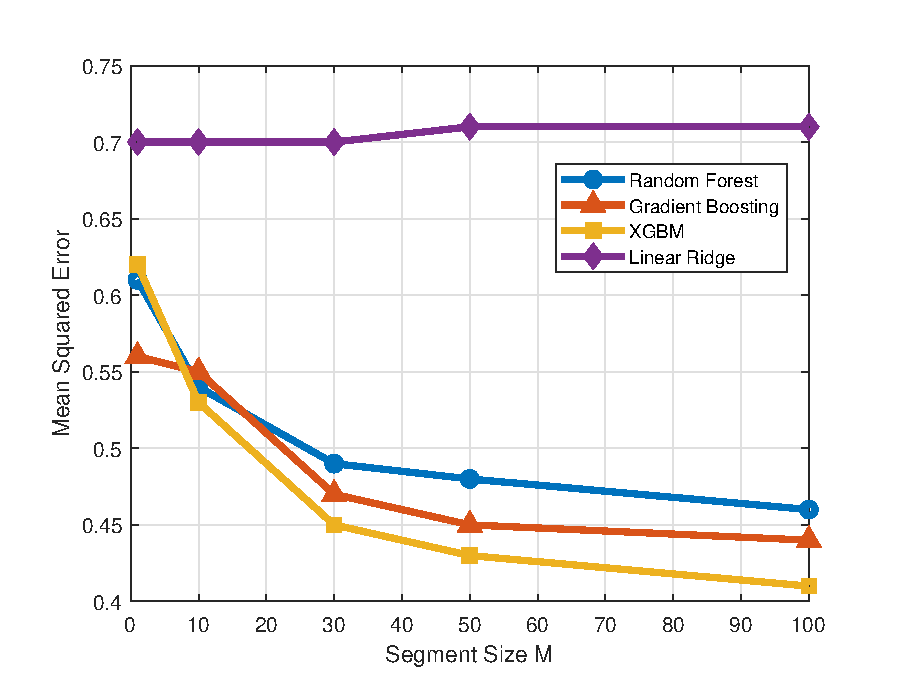
\includegraphics[width=0.75\columnwidth]{./chapter-ftml/plots/001_MSE_M.eps}
	\caption{The mean squared error performance for jamming setting b/g-Router of various algorithms against $M$.}
	\label{ftml-jrnl:fig:001_MSE_M}      
\end{figure}

In Fig.~\ref{ftml-jrnl:fig:001_R2_M}, we present the variance score for the same setting b/g-Router where a similar trend is found. The ensemble-based algorithms can achieves a variance score above 0.35 when $M$ is larger than 50. 

\begin{figure}[!ht]
	\centering
	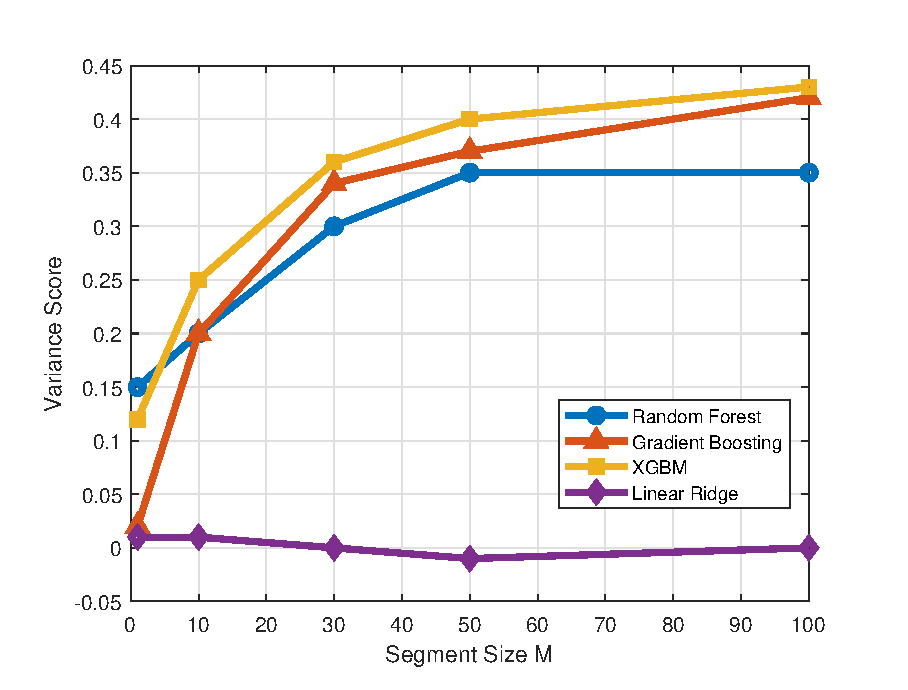
\includegraphics[width=0.75\columnwidth]{./chapter-ftml/plots/001_R2_M.eps}
	\caption{The variance score performance for jamming setting b/g-Router of various algorithms against $M$.}
	\label{ftml-jrnl:fig:001_R2_M}      
\end{figure}

In Fig.~\ref{ftml-jrnl:fig:002_MSE_M}, the MSE of the ensemble-based algorithms is shown for Setting b/g-Station where the router is impacted by the jamming signal. The MSE values in this setting are lower than those of setting b/g-Router where the predicted SIR values are smaller because the router has better capabilities to detect signals at lower SIRs.    
\begin{figure}[!ht]
	\centering
	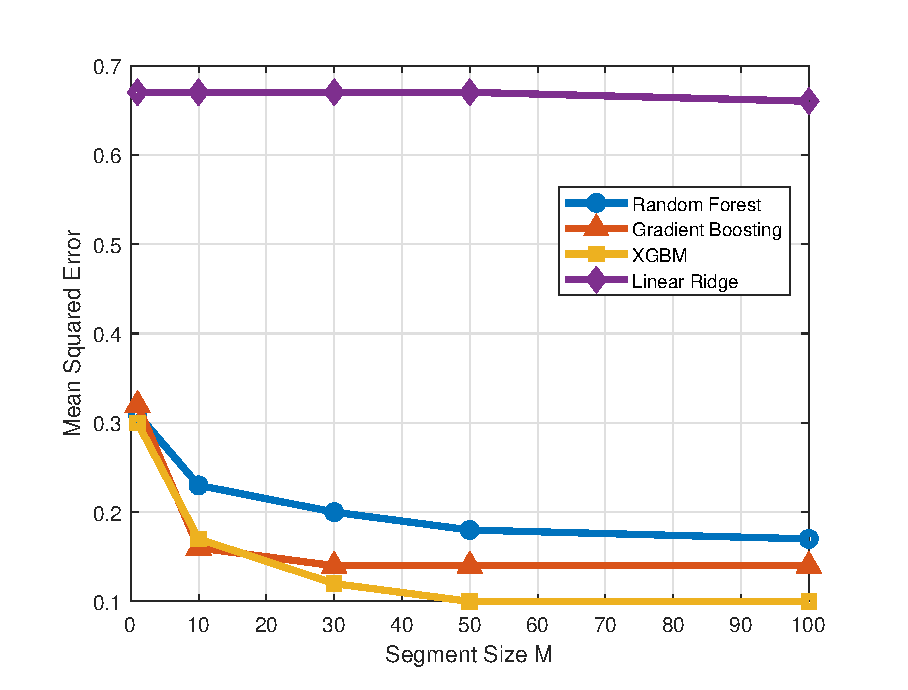
\includegraphics[width=0.75\columnwidth]{./chapter-ftml/plots/002_MSE_M.eps}
	\caption{The mean squared error performance for jamming setting b/g-Station of various algorithms against $M$.}
	\label{ftml-jrnl:fig:002_MSE_M}      
\end{figure}

Finally, in Fig.~\ref{ftml-jrnl:fig:004_MSE_M}, a similar scenario to Fig.~\ref{ftml-jrnl:fig:002_MSE_M} is presented where the router is impacted by the jamming signal. The difference is that at setting b/g/n-Station, a mixed IEEE802.11 b/g/n mode is allowed instead the IEEE802.11 b/g mode in setting b/g-Station. By allowing the IEEE 802.11n mode, the signal is more susceptible to interference and hence it is harder to predict the same SIR values. 

\begin{figure}[!ht]
	\centering
	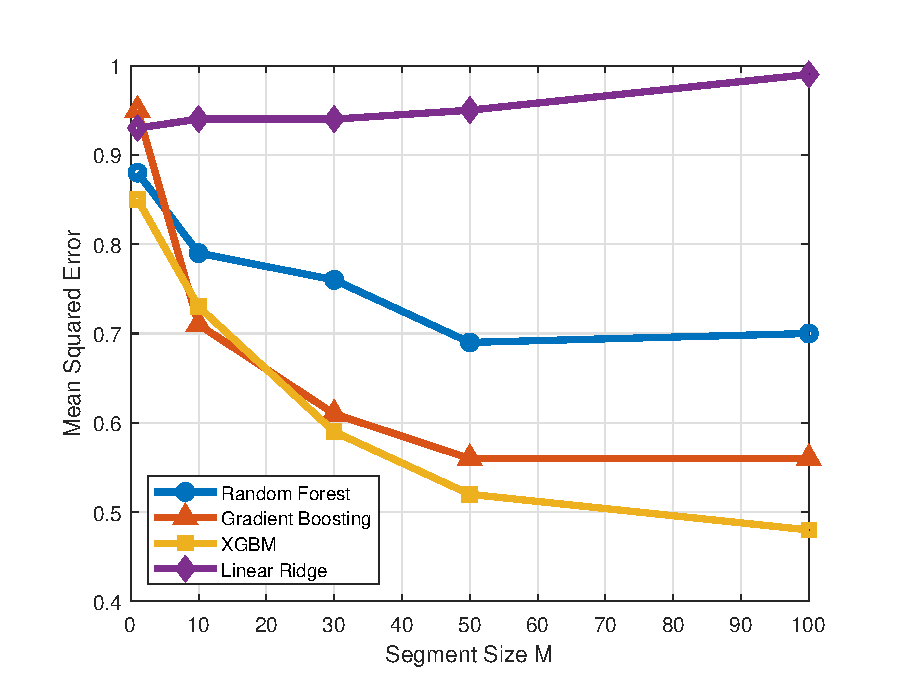
\includegraphics[width=0.75\columnwidth]{./chapter-ftml/plots/004_MSE_M.eps}
	\caption{The mean squared error performance for jamming setting b/g/n-Station of various algorithms against $M$.}
	\label{ftml-jrnl:fig:004_MSE_M}      
\end{figure}

\subsubsection{Impact of Training Sequence Length $T$}
In this subsection, we briefly discuss the impact of the training length on the performance of various algorithm. The parameter $T$ is the length of the training sequence where each element contains $M$ of the force seeking cycles. In the following figures, we show the MSE performance curves against $T$ for $M$ = 30 and 100. 

In Fig.~\ref{ftml-jrnl:fig:001_MSE_T}, increasing the training size $T$ can improve the prediction performance significantly. Gradient boosting and XGBM have higher improvement rate with $T$ than the random forest algorithm. 
%Moreover, in Fig.~\ref{ftml-jrnl:fig:004_MSE_T}, the random forest is almost not improving at all with $T$ because the prediction algorithm does not perform adequately in this case. 

\begin{figure}[!ht]
	\centering
	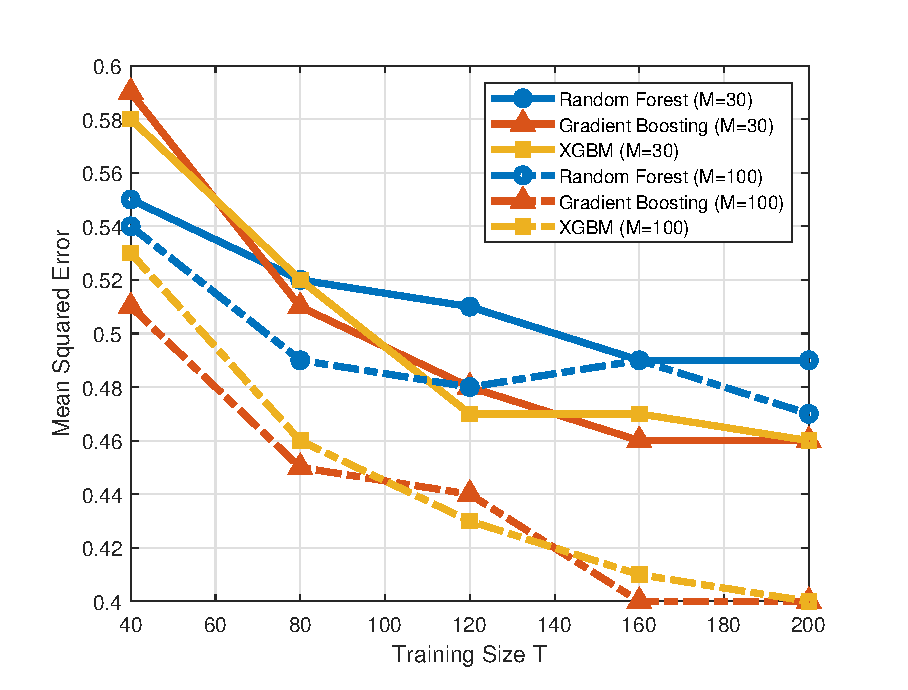
\includegraphics[width=0.75\columnwidth]{./chapter-ftml/plots/001_MSE_T.eps}
	\caption{The mean squared error performance for jamming setting b/g-Router of various algorithms against $T$.}
	\label{ftml-jrnl:fig:001_MSE_T}      
\end{figure}

% 			\begin{figure}[tbp]
% 	    \centering
% 		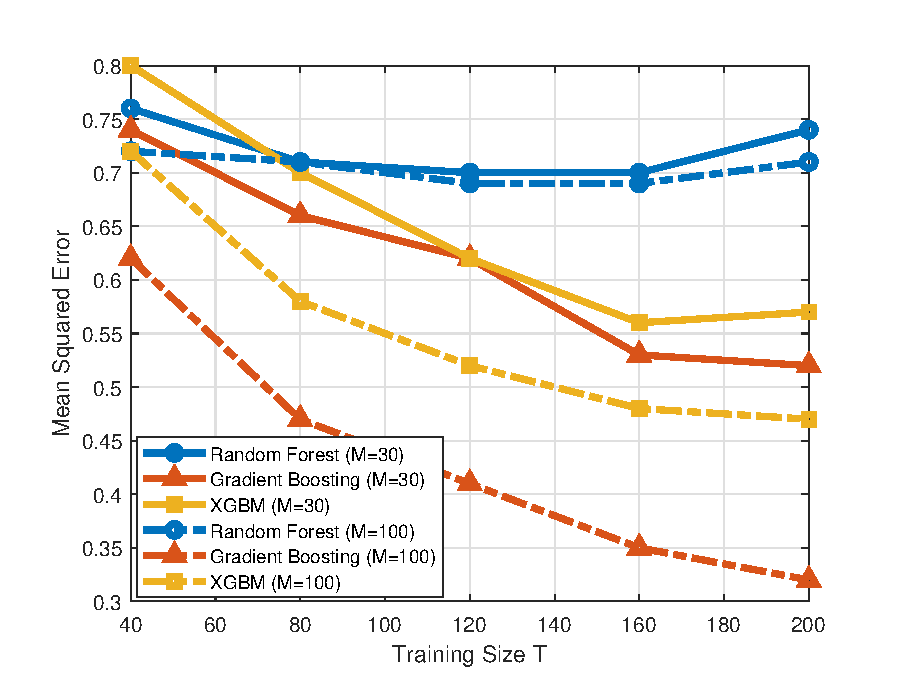
\includegraphics[width=0.8\columnwidth]{plots/004_MSE_T.eps}
% 		\caption{The mean squared error performance for setting 4 of various algorithms against $T$.}
% 		\label{ftml-jrnl:fig:004_MSE_T}      
% 	\end{figure}

\subsubsection{Impact of Individual Features}
In this subsection, we study the impact of the individual features on the performance of the ensemble-based machine learning algorithms. Understanding the importance of each feature on the prediction algorithms is essential in selection of features and hence reducing the required processing power for an algorithm. We show the results for XGBM algorithm for brevity and because the similarity of the behavior of various ensemble-based algorithms performance. 

In Fig.~\ref{ftml-jrnl:fig:001_MSE_F_3}, \ref{ftml-jrnl:fig:001_R2_F_3}, and \ref{ftml-jrnl:fig:004_MSE_F_3}, we present the MSE performance for setting b/g-Router, the variance score for setting b/g-Router and the MSE for setting b/g/n-Station, respectively, against the segment size $M$. In all the three figures, we refer to $\Delta{t}_{ab}$, $\Delta{t}_{bc}$, $Z_d$, $\Delta{t}_{cd}$, and $\Delta{t}_{ae}$ by "t\_high", "t\_plunge", "Descent Distance", "t\_bottom", and "Total Cycle", respectively. 

\begin{figure}[!ht]
	\centering
	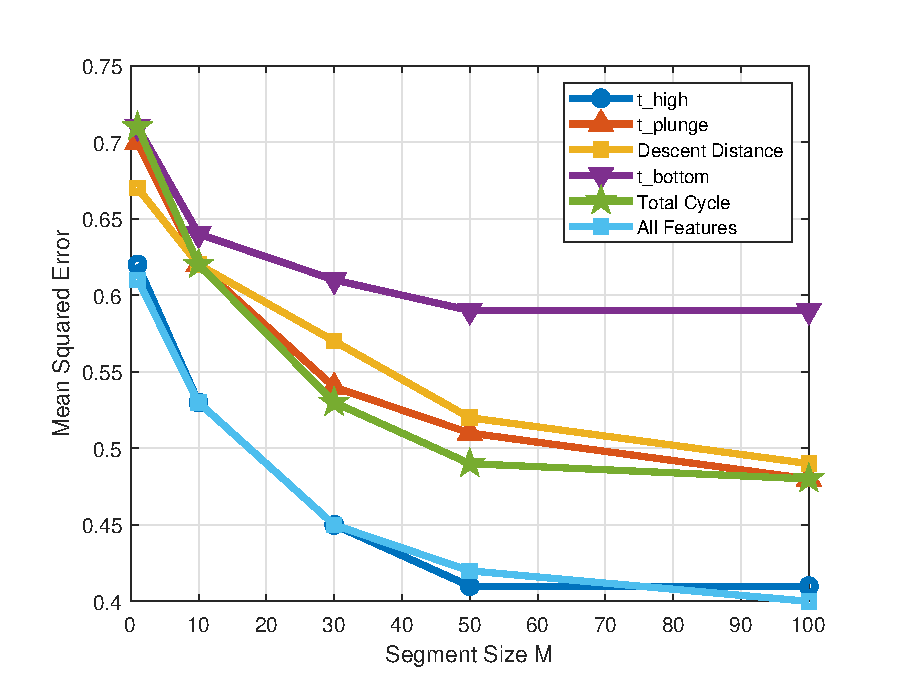
\includegraphics[width=0.75\columnwidth]{./chapter-ftml/plots/001_MSE_F_3.eps}
	\caption{The mean squared error performance for jamming setting b/g-Router of XGBM algorithm against $M$ including individual features impact.}
	\label{ftml-jrnl:fig:001_MSE_F_3}      
\end{figure}

\begin{figure}[!ht]
	\centering
	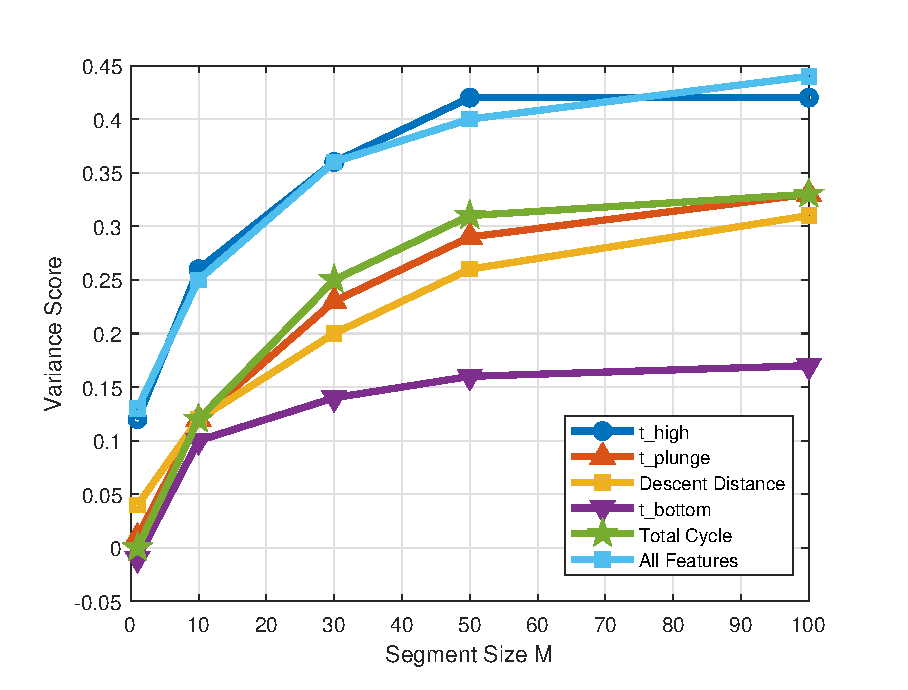
\includegraphics[width=0.75\columnwidth]{./chapter-ftml/plots/001_R2_F_3.eps}
	\caption{The variance score performance for jamming setting b/g-Router of XGBM algorithm against $M$ including individual features impact.}
	\label{ftml-jrnl:fig:001_R2_F_3}      
\end{figure}

\begin{figure}[!ht]
	\centering
	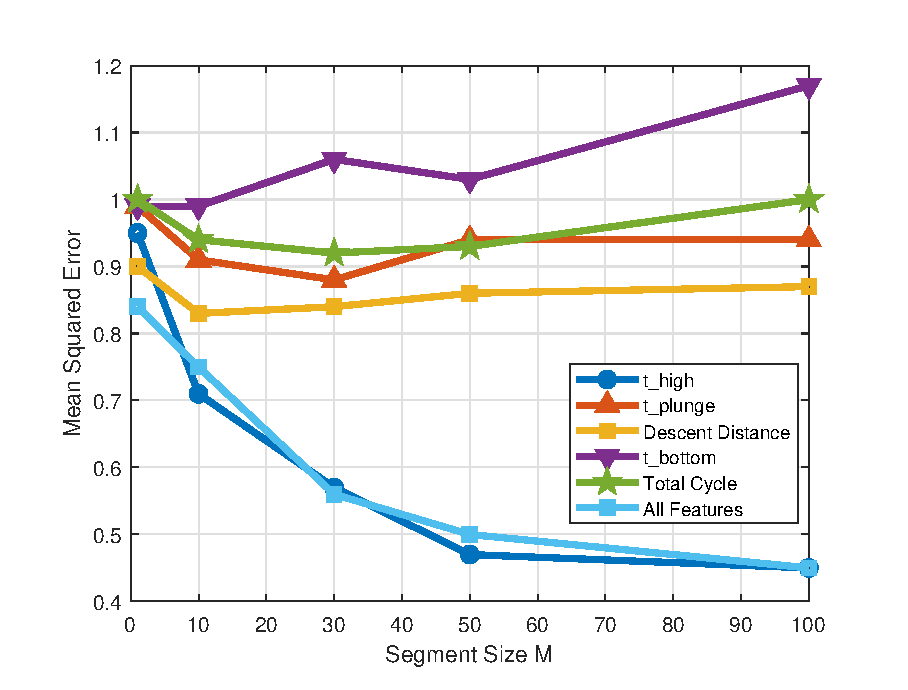
\includegraphics[width=0.75\columnwidth]{./chapter-ftml/plots/004_MSE_F_3.eps}
	\caption{The mean squared error performance for jamming setting b/g/n-Station of XGBM algorithm against $M$ including individual features impact.}
	\label{ftml-jrnl:fig:004_MSE_F_3}      
\end{figure}

The feature $\Delta{t}_{ab}$ is the most one impacted by the SIR value where the prediction performance by using this individual feature is almost identical to the performance of using all the features. This result can be explained by knowing that in the robot arm force seeking program, the FTS has to be zeroed before resuming the loop and hence there is a direct impact of the wireless transmissions and the value $\Delta{t}_{ab}$. On the other hand, the feature $\Delta{t}_{bc}$ is the least one impacted by the SIR value. This feature is defined as the reflection time of the robot arm to reverse its direction and hence it is minimally impacted by the SIR value. The rest of the features are impacted by the SIR to a certain level. Generally, adding an unnecessary feature can degrade the performance. As a result, in this work, we concluded that using $\Delta{t}_{ab}$ can substitute all the five features to get the same MSE and variance score performance with much less processing.

\subsection{Conclusion}\label{ftml-jrnl:sec:conclusion}

In this paper we have presented a practical use case of a wireless force-torque feedback control system that could be deployed in a manufacturing assembly system such as a pick-and-place or assembly operation.  A 6-DOF force-torque sensor was connected to a robot controller tasked with moving a probe along a linear path until an opposing force exceeding 5 N was detected.  We demonstrated that the reliability of the wireless communication system directly impacts the repeatability performance of the physical system. We also demonstrated that the quality of the underlying wireless channel may be inferred by observing the position of the probe along a single spatial dimension and applying machine learning to predict the signal-to-interference ratio. As a result of our exploration of various machine learning algorithms on the prediction of signal quality, we found that ensemble-based algorithms have superior performance compared to other regression algorithms for data presented.  Additionally, our analysis shows that careful study of the MSE and variance score is useful in selection of features used for training the algorithms. We conclude for this particular force-torque control system scenario that the dwell time of the robot before descending was the most useful feature for training the algorithm. Our findings provide motivation for applying machine learning to larger more complex systems with higher degrees of freedom. We conclude by stating that future  experimentation with neural networks and deep learning to improve prediction accuracy could be of value to improving the reliability of wireless operations in factories. The applications of online machine learning techniques to this and other use cases could provide significant benefits to the manufacturing community through integration of link quality detection with programmable controllers.
